\documentclass[12pt]{article}
\usepackage{xeCJK}%preamble part
\usepackage{graphicx}
\usepackage{multirow}
\usepackage{pdfpages}
\usepackage{indentfirst}
\usepackage[a4paper, inner=1.5cm, outer=3cm, top=2cm, bottom=3cm, bindingoffset=1cm]{geometry}
\usepackage{epstopdf}
\usepackage{listings}
\usepackage{array}
\usepackage{color}
\usepackage{fontspec}
\usepackage{caption}
\usepackage{subcaption}
\usepackage{bm}
\usepackage{gensymb}
\usepackage{todonotes}
\usepackage{amsmath, amsthm, amssymb}
\usepackage[citecolor=blue]{hyperref}
\newtheorem{definition}{Definition}
\newtheorem{thm}{Theorem}[section]
\newtheorem{cor}[thm]{Corollary}
\newtheorem{lem}[thm]{Lemma}
\DeclareMathOperator{\sgn}{sgn}
\theoremstyle{remark}
\newtheorem*{rem}{Remark}
\usepackage{makecell}
\setCJKmainfont[BoldFont={SimHei}]{SimSun}
\setCJKmonofont{SimSun}
\setmainfont{Times New Roman}
\newCJKfontfamily[hei]\heiti{SimHei}
\setlength{\extrarowheight}{4pt}
\setlength{\parindent}{1cm}
\definecolor{codegreen}{rgb}{0,0.6,0}
\definecolor{codegray}{rgb}{0.5,0.5,0.5}
\definecolor{codepurple}{rgb}{0.58,0,0.82}
\definecolor{backcolour}{rgb}{0.95,0.95,0.92}
\lstdefinestyle{mystyle}{
    backgroundcolor=\color{backcolour},
    commentstyle=\color{codegreen},
    keywordstyle=\color{magenta},
    numberstyle=\tiny\color{codegray},
    stringstyle=\color{codepurple},
    basicstyle=\footnotesize,
    breakatwhitespace=false,
    breaklines=true,
    captionpos=b,
    keepspaces=true,
    numbers=left,
    numbersep=5pt,
    showspaces=false,
    showstringspaces=false,
    showtabs=false,
    tabsize=2
}

\lstset{style=mystyle}
\begin{document}
\title{\textbf{\fontsize{15.75pt}{\baselineskip}{抛物型方程实验}}}
\author{数33 赵丰 \\学号:2013012178}

\maketitle
\large
\section{题目}
\includepdf{practice4.pdf}
\section{数值格式}
结合算子分裂和交替方向隐式的格式构造如下具有二阶精度且无条件稳定的差分格式:
\begin{eqnarray*}
% \nonumber % Remove numbering (before each equation)
  u_{jk}^{n+1/3}-u_{jk}^{n} &=& \frac{\lambda}{2}(\delta^2_x u_{jk}^{n+1/3}+\delta^2_yu_{jk}^{n}) \\
  u_{jk}^{n+2/3}-u_{jk}^{1/3+n} &=& \frac{\lambda}{2}(\delta^2_x u_{jk}^{n+1/3}+\delta^2_yu_{jk}^{n+2/3}) \\
  \ln|\frac{u}{\sqrt{1-u^2}}|\biggr\rvert^{u_{jk}^{n+1}}_{u_{jk}^{n+2/3}}&=&\frac{\tau}{\epsilon}
\end{eqnarray*}
其中采用解析解处理ODE可以保证整个格式二阶精度且无条件稳定。
以下是采用如上数值格式的Mathematica代码,通过函数式编程使得代码量大大减少
\begin{lstlisting}[language=Mathematica]
(*Initialization*)
a = 0.8;
b = 0.6;
\[Epsilon] = 0.1;
\[Tau] = 0.02;
h = 0.1;
\[Lambda] = \[Tau]/h^2;
f[x_] := Log[Abs[x/Sqrt[1 - x^2]]]
u0 = Table[
   If[(x/a)^2 + (y/b)^2 <= 1, 1, -1], {y, -1, 1, h}, {x, -1 + h,
    1 - h, h}];
L = Length[u0] - 2;
m = SparseArray[{Band[{1, 2}] -> -\[Lambda]/2,
    Band[{1, 1}] -> 1 + \[Lambda], Band[{2, 1}] -> -\[Lambda]/2}, L];
(*Iteration from tn to t(n+1)*)
For[i = 1, i*\[Tau] < 1, i++,
 RHS = \[Lambda]/2*Differences[u0, {2, 0}] + u0[[2 ;; (L + 1)]];
RHS[[;; , 1]] -= 1;
RHS[[;; , -1]] -= 1;
 un13 = Transpose[LinearSolve[m, #] & /@ RHS];
 PrependTo[un13, Table[-1, {i, L}]];
 AppendTo[un13, Table[-1, {i, L}]];
 un13RHS = \[Lambda]/2*Differences[un13, {2, 0}] +
un13RHS[[;; , 1]] -= 1;
un13RHS[[;; , -1]] -= 1;
   un13[[2 ;; (L + 1)]];
 un23 = Transpose[LinearSolve[m, #] & /@ un13RHS];
 un33 = Sqrt /@ (1 -
     1/(1 + (Exp /@ (\[Tau]/\[Epsilon] + f /@ un23))^2));
 PrependTo[un33, Table[-1, {i, L}]];
 u0 = Append[un33, Table[-1, {i, L}]];
 ]
\end{lstlisting}
下图是在t=1时$[-1,1]\times[-1,1]$区域内$u(x,y)$的取值:
\newpage
\begin{figure}[!ht]
  \centering
	\begin{subfigure}[t]{.5\linewidth}
		\centering
		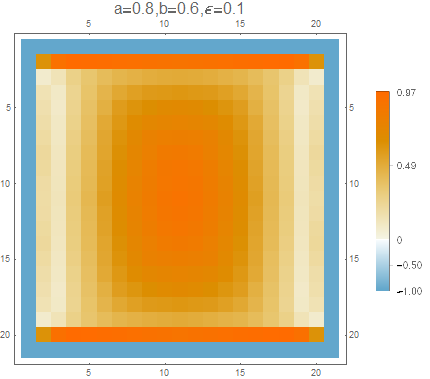
\includegraphics[width=230pt]{matrixPlot1.png}
	\end{subfigure}
	\quad
	\begin{subfigure}[t]{.3\linewidth}
		\centering
		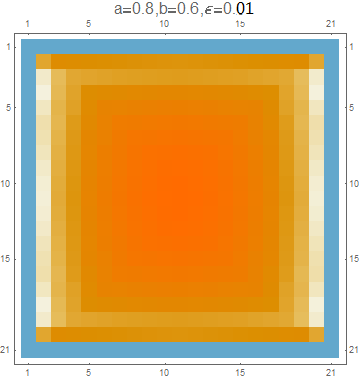
\includegraphics[width=200pt]{matrixPlot2.png}
	\end{subfigure}
\end{figure}

由上图可以看出
\begin{itemize}
\item 短轴(b<a,y)方向扩散的更快,使得y方向更快的接近1;
\item $\epsilon$越小反应速率越快,使得在相同时间(t=1)时,右图大部分区域更接近1;
\item 由于边界条件恒取-1,所以在扩散和边界之间会有突变,但x,y方向边界层特性不同,短轴方向几乎是从-1到1的突变而长轴方向有0的过渡。
\end{itemize}
如果进一步加密空间网格,则可以观察到如下图所示的现象:

\begin{figure}[!ht]
  \centering
  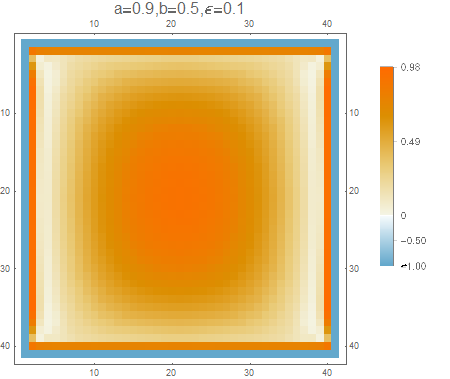
\includegraphics[width=270pt]{matrixPlot3.png}
\end{figure}

边界-1的外层被接近1的一层包围,内部是正常的扩散衰减现象。
\end{document}
